
\subsection{Setting up the Simulation}

Given the Hamiltonian \ldots in \ldots it
is possible to evolve the system
according to the schrodinger
equation. However since we
are only interested in the
evolution of the eigenstates
at times much greater than
the frequency of the sates
\(\omega = \frac{E}{\hbar}\)
it is better to first
break up the initial
state into the eigenstates
of the Hamiltonian
before applying the
relevant phase to
each eigenstate
\begin{align}
    \ket{\Psi(t)} = \exp{(-i\frac{Ht}{\hbar})} \sum_n C_n \ket{n} \\
    = \sum_n C_n \exp{(-i\frac{E_n t}{\hbar})} \ket{n}
\end{align}

TODO Code Snippet


One possible issue with this method
is the

storing the eigenstates, however
\ldots the cost of

In general it is difficult to produce
a hamiltonian which \ldots spin
statistics of the fermion,
however since our Hamiltonian is
described using only
pairs of creation and annihilation
operators it is relatively easy to
cast it into matrix form

Although in general \ldots hard to write
a hamiltonian for fermions \ldots
since our hamiltonian was formed.

Once the eigenvalues and eigenvectors of the
matrix were found an arbitrary state could
be evolved in time by decomposing into by the hamiltonian

\subsection{}
Since the Hamiltonian conserved particle number
it was possible to restrict the electron basis
to states for which the total number of electrons
was constant.
\ldots electrons are fermions we either had 1 or
0 electrons
\ldots table of number of states


However in practise larger matrix elements
also had a larger cost associated with
the time evolution of
the eigenstates, and as such we limited ourselves
to at most \(10\) energies and \(5\) electrons,
corresponding to \(504\) total states.

\subsection{Choosing the Initial States}

\subsubsection{Distribution Of Energies}
The distribution of electron energies

To prevent these oscillations random offsets were introduced
into the electron energy distribution, and after
averaging over several runs almost all of the
noise could be eliminated from the plot.

The spacing of electron energies is also
important for the simulation, as it
sets the effective volume of the Nickel
lattice. The density of states of a free electron
gas \(g(E)\) is given by~\cite{KittelCharles1953Itss}
\begin{equation}
    g(E) = \frac{V}{2\pi^2}
    {(\frac{2m}{\hbar^2})}^{\frac{3}{2}}
    E^{\frac{1}{2}}
\end{equation}
We therefore invert this expression
to find the implied volume of the
simulation
\begin{equation}
    V = 2\pi^2
    \frac{g(E)}{E^{\frac{1}{2}}}
    {(\frac{\hbar^2}{2m})}^{\frac{3}{2}}
\end{equation}
Since at large \(k\)
(for \(k\sim k_f\))
the density of states is roughly
constant we make the approximation
\begin{equation}
    g(E) = \frac{dN}{dE} \sim \frac{1}{E_{space}}
\end{equation}
where \(E_{space}\) is the energy spacing
of the simulation.
If we look at the expression for the
interaction hamiltonian


For smaller
energy spacing we therefore have
a larger volume, and a smaller
perturbation.

---

---

It was however not possible to
reduce the electron spacing to
below \ldots
TODO -BAndwidth justification.
however as we decrease the electron
spacing we also increase the tunnelling
times, as we choose to sample fewer and
fewer electrons \ldots so this is not seen.

\subsubsection{Distribution Of Electrons}
To be able to average over successive
simulations we also need to setup the
simulation with a somewhat random
choice of initial states. Since the states
are represented by vectors in a 2N dimensional
vector state \ldots a. To start the electron
in the \(FCC\) site we therefore set the
amplitudes of the \(HCP\) sites to zero
and choose the \(FCC\) aptitudes according to
a normal distribution before normalising.

In simulations for which we choose states
with a large range of energies however
the electron distribution should not be
random and should follow the fermi dirac distribution.
To match this distribution at \(T=0\) we therefore
need to alter the averages used
to produce the initial state vector.
Since the amplitude corresponds to
the square-root of the probability we
take the average magnitude as the
square-root of the boltzmann probability
associated with each state.
\begin{align}
    P_k & = \exp(-\beta{}E_k)     \\
    C_k & = \exp(-\beta{}E_k / 2)
\end{align}
If we plot the resulting
electron distribution produced
by this method for fixed N however
we do not see the expected electron
distribution for a standard electron
gas.
TODO-PLOT THIS

This is because the
derivation assumes a distribution
of states at all N, weighted by the
chemical potential. If we add back
these states we find that the correct
distribution is recovered.
TODO-Plot
In most cases we choose to
simulate only the most
likely configuration of electrons,
assuming the chemical potential is large.
This holds for all but the state at
\(k = k_f\) where we have \(\mu = 0\)
relative to the average energy of the
electrons. However the number of
states \ldots \(ACB\) big for N=2
TODO-section correcting for this effect!!!


This approach however does not take
into accounts the shift in energies
caused by the perturbation. This
does not effect the distribution
for a small perturbation,
however in some cases,
especially those for which the energy
spacing was large this assumption
no longer holds. In this case
we see the electron distribution
begin to diverge from the
boltzmann distribution at large times.
TODO-Plot


Full code is available in the appendix TODO-






\subsection{Initial Investigation}
To obtain a rough estimate of
the rate the system was setup
with electrons evenly spaced
in the region \(E_k = E_f \pm 2K_b T\)
with degenerate hydrogen energies.

\begin{figure}[htb]
    \centering
    \begin{subfigure}{0.45\linewidth}
        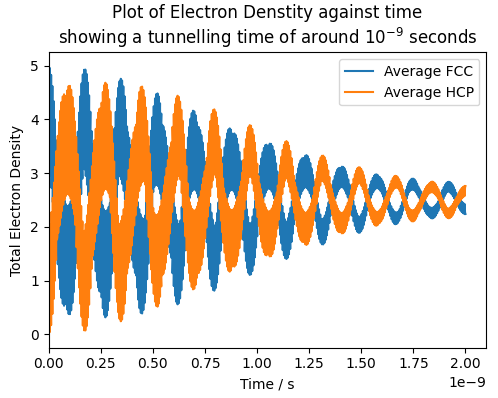
\includegraphics[width=0.9\linewidth]{Figures/Simulation/Plot of large band simulation decay times.png}
        \subcaption{Tunnelling excluding hydrogen energy}\label{fig:large band degenerate simulation}
    \end{subfigure}
    \begin{subfigure}{0.45\linewidth}
        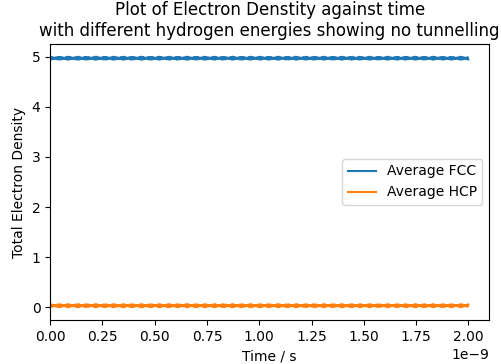
\includegraphics[width=0.9\linewidth]{Figures/Simulation/Plot of large band simulation with hydrogen energies.png}
        \subcaption{Tunnelling including hydrogen energy}\label{fig:large band non degenerate simulation}
    \end{subfigure}
    \caption{Plot of the tunnelling rate taken using a
    simple choice of electron energies,
    taken evenly in the range \(E=E_f \pm K_b T\).
    Simulation with a degenerate hydrogen
    (\cref{fig:large band degenerate simulation})
    shows tunnelling in around
    \(3\times{}10^{-10}s\), however when the
    hydrogen energy is included (\cref{fig:large band non degenerate simulation})
    no tunnelling can be seen, even
    at much larger timescales.}
\end{figure}

Since we are choosing electrons
with a relatively large spacing
we have large
interaction. The diagonal terms in
the interaction hamiltonian
had a value of \(1.03\times{}10^{-21}J\)
and a cross diagonal value of \(4.53\times{}10^{-23}J\)
whereas the electron energies were separated
by only \(2.3\times{}10^{-22}J\). This meant that
the perturbation approximation required for
fermi dirac distributed states is not valid TODO PLOT TEMP inversion.
Luckily however in the region \(\pm K_b T\)
the electron distribution is relatively flat,
and this should therefore have very little
effect on the tunnelling rate.

\subsection{Differing Hydrogen Energy}
If we add the hydrogen energies to the
simulation we no longer see tunnelling
on any timescale. This is caused by the
principle of energy conservation --- tunnelling
TODO-Band Diagram

If we employ the uncertainty principle
\(\Delta{}E\Delta{}T \geq \frac{\hbar}{2}\)
we expect the total energy to be conserved
to within
\begin{equation}
    \Delta{}E \sim \frac{\hbar}{2\Delta{} t}
\end{equation}
for a tunnelling time of \(\sim 10^{-10}s\)
we would expect an energy fluctuation
of \(\sim 5\times{}10^{-25} J\).


. Since tunnelling occurs between sates which are
degenerate in energy \ldots we don't see any tunnelling

Using the energy time uncertainty principle
\(\Delta{}E\Delta{}T \geq \frac{\hbar}{2}\), and
using a tunnelling time of \(\sim 10^{-9}s\) TODO-CITE
we are able to identify that no significant tunnelling
can occur between states separated by more than
\(\Delta{}E \sim 5\times{}10^{-26} J\). This is
much smaller than the range of energies for
which the electrons are able to undergo
transitions about the fermi surface
(\(K_b T \sim 2 \times 10^{-21}J\) at \(150K\)).


\ldots when choosing states evenly in this
range we only see degenerate tunnelling

\section{Multi Band Approach}
To resolve these issues we instead simulated the system
taking the basis of electrons placed in two bands,
with each band separated by the hydrogen energy
difference.
with
the states in each band separated by at most \ldots.


When applying this approach however very
little tunnelling of the hydrogen is seen at all timescales.
Look at the energy distribution almost all
of the HCP electrons lie in the lowest energy band.
This corresponds to a system with a much lower
temperature than the initial condition.
The lack of tunnelling can therefore be explained
\ldots and if
the final states were to lie in a boltzmann  distribution
this would explain the lack of tunnelling

Running the simulation
in reverse (from HCP to FCC) the electrons
distribution \ldots population inversion.
The heat bath is therefore much to small
to accommodate the energy difference of
the two hydrogen sites.

TODO- fermi distribution
TODO- tunnelling curve
..It is therefore impossible to measure a tunnelling
rate.

TODO- The rate of tunnelling might also
be much different at such a low temperature,
and as such it is impossible to say if
any of these results would be valid
for the real system.

\subsection{Degenerate Correction Approach}
From the previous investigation it is clear
that it is not possible to incorporate the
hydrogen energy directly \ldots. In the
real system the electrons would move
between states at a much shorter time
period than that of hydrogen tunnelling.
After an electron transitions to a lower
band the fermi distribution should therefore
be recovered almost instantaneously. We
therefore `fix' the behaviour by
ignoring the fact the electron
has moved to a lower band at all,
allowing tunnelling of the hydrogen
which leaves the electron distribution
untouched. This is exactly what
we see in a system when we ignore
the hydrogen energy difference.


The Approach used to simulate the system is as follows

\subsection{Correcting for unfixed N}